\documentclass[journal]{IEEEtran}

\usepackage{cite}
\usepackage{amsmath}
\usepackage{graphicx}
\usepackage{booktabs}
\usepackage{hyperref}
\usepackage{url}
\usepackage{tabularx}
\usepackage{tfrupee}
\usepackage{tikz}
\usepackage{float}
\usetikzlibrary{shapes.geometric, arrows.meta, positioning, calc}

% === TikZ Workflow Styles (IEEE column-width safe) ===
\tikzset{
  wf node/.style={
    rectangle, rounded corners=2pt, draw=black, fill=gray!8,
    text width=1.3cm, minimum height=0.65cm,
    text centered, font=\sffamily\scriptsize,
    inner sep=2pt
  },
  wf trigger/.style={
    wf node, fill=gray!20, font=\sffamily\scriptsize\bfseries
  },
  wf decision/.style={
    diamond, draw=black, fill=gray!8,
    text width=0.7cm, minimum height=0.5cm,
    text centered, font=\sffamily\scriptsize,
    inner sep=1pt, aspect=2.2
  },
  wf arrow/.style={
    -Stealth, thick, draw=black!70
  },
  wf label/.style={
    font=\sffamily\tiny, fill=white, inner sep=1pt
  }
}

\hypersetup{
    colorlinks=false,
    pdfborder={0 0 0},
}

\begin{document}
\raggedbottom

\title{StockSense AI: Intelligent Inventory for India's Small Retailers}

\author{Vyshakh Vijayan%
\thanks{Vyshakh Vijayan is with the Department of Computer Science and Business Systems, VIT-AP University, Amaravati, Andhra Pradesh, India. Email: vijayan.22bcb7055@vitapstudent.ac.in}%
}

\markboth{StockSense AI Project Report}%
{Vyshakh Vijayan: StockSense AI: Intelligent Inventory Management for Small Retail Stores}

\maketitle

\begin{abstract}
Most of the small scale shop owners or kirana Store owners still use notebooks or at max Excel sheets to track their inventory. They don't have access to  tools or technologies which help them in tracking the inventory and predicting situations like stockouts etc. Also, using the large scale expensive enterprise software is really impractical for them.

In order to solve this problem I developed StockSense AI, which is an intelligent inventory management tool for the small retailers. It can predict stockout dates, flag risky items, score suppliers using a Weighted Sum Model, and explain generate reorder decisions along with it's explanation using the assistance of an LLM. Finally,the alerts generated will be sent directly to the shop owners WhatsApp.

The entire product can be automated by enabling the orchestration of the pipeline at a fixed time so that the inventory is up to date. The product is powered  by 10 individual N8N workflows, which act as the brain of the system.
\end{abstract}

\begin{IEEEkeywords}
Inventory Management, Supply Chain Intelligence, Workflow Automation, n8n, Large Language Model, Supplier Scoring, Kirana Stores, SME Technology
\end{IEEEkeywords}

\section{Introduction}
\IEEEPARstart{T}{here} are 12 million kirana stores in India and they act as the supporting pillar of the retail industry in our country. But most of them face the common problem of efficient inventory management. They have to deal with situations like stockouts where they can loose a potential customer and overstock situations which is again financial loss.

Small retailers face a specific set of constraints. Suppliers are scattered and unreliable. Delivery times change without warning. Affordable tools do not exist. Enterprise ERP costs thousands per month and is too complicated for one person to operate. Most point-of-sale systems only record what was sold. They do not predict what will be needed, warn about stockouts, rank suppliers, or recommend reorders.

I built StockSense AI to fill this gap. The system tracks inventory levels and projects stockout dates using daily sales velocity. It extracts product details and processes supplier invoices from photos using Google Gemini 2.5 Flash. It generates reorder suggestions using Groq Llama 3.1 8B. It ranks suppliers based on price, reliability, and delivery speed. It sends alerts directly to the shop owner's WhatsApp. And it runs on a nearly free infrastructure that requires no manual setup.

\section{Related Work}

Researchers have built inventory systems using IoT sensors, RFID tags, and cloud platforms. But adoption remains low among small businesses. Enterprise solutions cost thousands per month and require IT expertise most store owners don't have.

Machine learning can forecast demand better than simple moving averages. That's well-known. The catch is that implementing machine learning requires skilled engineers and infrastructure that small retailers can't afford.

Recently, large language models have been proposed for procurement and ordering. They can reduce human bias in decision-making. But I found very little published work on running LLMs in real-time operational workflows with tight cost constraints. That gap is what I wanted to address.

Low code platforms like N8N has changed the overall technical capabilities and oppurtunities. Before this people had to hire an experienced developer to build workflow automation's for businesses, but nowadays people with even less or no technical knowledge can build automation workflows for various needs.

The supplier scoring model used in this project is also not a new concept as it is a fundamental concept of ranking suppliers based on pricing, reliability and delivery speed that has been used in the field of supply chain management and operations research for many decades.

All the concepts discussed above exists as individual systems and they are used in various industries, but a complete package of all of them tied together as a single system is something which is missing and will be really helpful for small scale shop owners as they don't require the complex retail solutions available in the market which comes along with expensive hardware's like barcode scanner, RFID readers etc.Implementation of such heavy systems will be unnecessary financial burden on the kirana shop owners.
  
The approach that I used here is very simple. I am not claiming that I have built a complex software system, but what I have built is a very simple automation based system based on N8N which involves features like daily inventory management, stock alerts, supplier scoring, WhatsApp alerts, AI enabled inventory processing etc. This is a simple solution for the daily inventory related problems that kirana show owners face.

\section{Motivation and Problem Specification}

My main motivation is to address the significant gap that exists between the high end enterprise solutions available in the market and the actual ground reality of operational conditions of small scale retailers in the country.

\subsection{Socio-Economic Motivation}
Kirana shop owners comprises over 50 percentage of India's retail market and it clearly shows that they contribute significantly towards the growth of the country. They operate in a very dynamic environment where situations like stock out or overstock can significantly impact them financially. Due to their limited budget and lack of technical staff, it is very difficult for them to afford high end enterprise solutions available in the market. Hence, the primary objective of StockSense AI is to make sure that even small scale shop owners have access to inventory intelligence without needing to subscribe to expensive ERP solutions.

\subsection{Gap Analysis and Technical Advantage}
A comprehensive analysis on this problem shows that there are two major gaps in the existing system:
\begin{enumerate}
    \item \textbf{Financial Barrier}: Most of the existing solutions require expensive hardware like barcode scanners and they are really expensive for small scale business owners.Whereas StockSense AI operate under Rs.500/month by making use of free tier or low cost cloud services.
    \item \textbf{Intelligent Support}: Basic POS systems that are available in the market can show what was sold but they cannot predict what will be needed or stockout conditions very efficiently. Hence, the integrating the LLM model provides a reasoning based reorder logic that was previously available to only large scale retail chains. 
\end{enumerate}

\subsection{Problem Statement}
The main objecive of my project is to design and implement a system that require minimum infrastructure needs and operate with the help of a automated intelligence pipeline that provides a really advanced inventory management system for small scale shop owners with features like stock our alerts delivered through WhatsApp, AI based reorder suggestions etc. 

\section{Proposed System}

\subsection{System Architecture}

The system basically consists of 4 main layers with  different responsibility and they communicate with each other with the help of REST API framework. This current design ensures that the overall system is modular, scalable and easier to test.

The \textbf{Frontend Layer} is built using tech stack like React 19, Vite 8 and Tailwind CSS v4. The user can see various interfaces like an invntory dashboard showing current stock levels and overall store health, AI based reorders suggestions page, supplier scoring page etc. The frontend communicate with the backend that is N8N workflow automations using REST webshooks and connects to supabase for authentication and real time updates.

The \textbf{Workflow Engine Layer} is based on a latest technology called N8N, which is an open source automation platform. There are 10 different workflows in this project that handles various functions like:

\begin{itemize}
\item \textit{WF-01} (Data Ingestion): Takes care of the inventory updates and delivery records in the database.
\item \textit{WF-02} (Stockout Calculation): Calculates days to stockout for each product.
\item \textit{WF-03} (Alert Filtering): Highlights risky products with stock level below their threshold.
\item \textit{WF-04} (Risk Scoring): Classifies risk levels of products as HIGH, MEDIUM, LOW, or UNKNOWN.
\item \textit{WF-05} (AI Suggestions): Generate reorder recommendations with the help of Groq AI.
\item \textit{WF-06} (Supplier Scoring): Calculates supplier score using  the Weighted Sum Model.
\item \textit{WF-07} (WhatsApp Delivery): Sends stock alerts to the shop owners with the help of Twillio API.
\item \textit{WF-08} (Master Orchestrator): When deployed in cloud it will run daily automatically at a fixed time executing WF-02 to WF-07 in a sequential order.
\item \textit{WF-09} (AI Vision Onboarding): Extracts product details automatically using Gemini 2.5 Flash model and helps in updating product details.
\item \textit{WF-10} (Smart Scan Invoices): Process supplier bills using Gemini 2.5 Flash to automatically update stock levels.
\end{itemize}

The \textbf{Database Layer} uses Supabase which is an open source postgreSQL based development platfom that provide real time access via websockets. The project schema consists of 8 major tables like Store Profile, Products, Suppliers, Stock Alerts, Reorder Suggestions, Stock Transactions, Daily Snapshots and System Logs. When the pipeline runs and inventory or alerts change the real time subscription pushes the latest updates to the frontend ensuring that there is no stale data.

The \textbf{AI/External Services Layer} integrates three external APIs. First one is the Groq's Llama 3.1 8B model that help in generating reorder reasoning, second is the Google Gemini 2.5 Flash model that helps in image based product and invoice processing, and last one is Twilio's WhatsApp Business API that helps in sending alerts to the shopowners. In WF-05,product data, stock levels, and supplier information is passed to Groq, it then processes all the inputs and give a reorder suggestion with reason. In WF-09 and WF-10, Gemini extracts structured data from the uploaded product or invoice images. In WF-07, alerts are generated and sent to the shopowners WhatsApp as soon as the pipeline runs.

All layers communicate with eachother using HTTP REST and standard database drivers. Hence, it facilitate easy testing of each layers independently without affecting another.

\begin{figure}[H]
\centering
\resizebox{\columnwidth}{!}{%
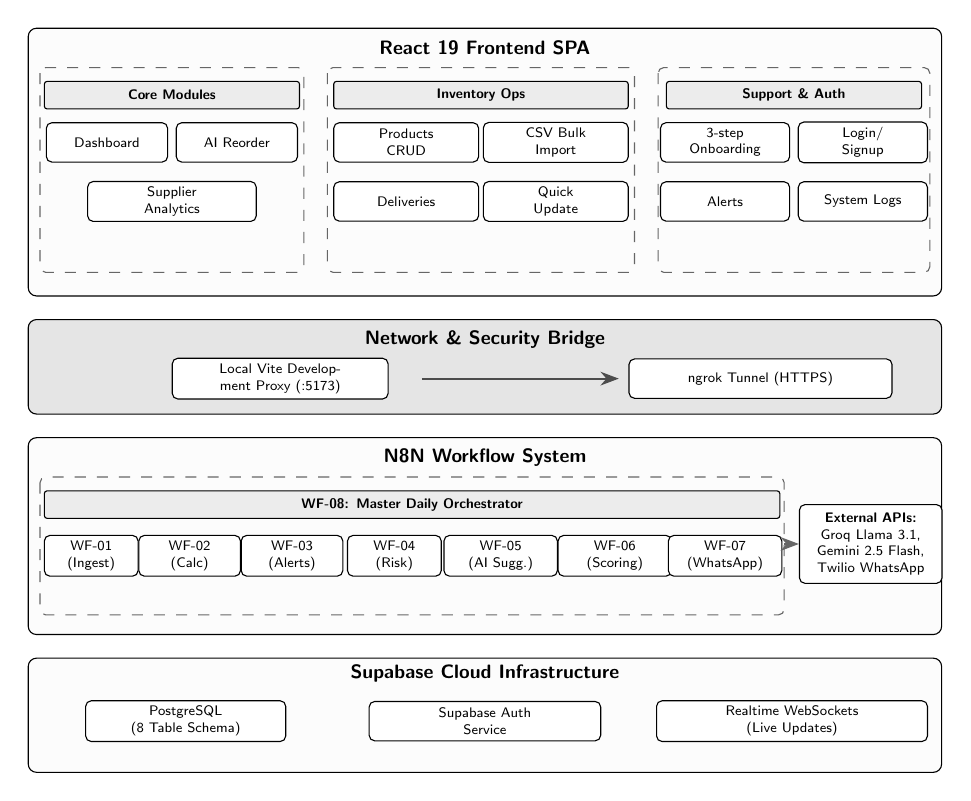
\begin{tikzpicture}[align=center,
  md/.style={rectangle, rounded corners=2pt, draw=black, fill=white,
    font=\sffamily\tiny, minimum height=0.5cm, text centered, inner sep=2pt},
  hd/.style={rectangle, rounded corners=1pt, draw=black, fill=gray!15, 
    font=\sffamily\tiny\bfseries, minimum height=0.35cm, text centered, inner sep=2pt},
]

% ====== LAYER 1: React 19 Frontend SPA ======
\draw[black, rounded corners=3pt, fill=gray!2] (0,0) rectangle (11.6,-3.4);
\node[font=\sffamily\scriptsize\bfseries] at (5.8,-0.25) {React 19 Frontend SPA};

% -- Core Modules --
\draw[black!60, rounded corners=2pt, dash pattern=on 4pt off 4pt] (0.15,-0.5) rectangle (3.5,-3.1);
\node[hd, text width=3.1cm] at (1.825,-0.85) {Core Modules};
\node[md, text width=1.4cm] at (1.0,-1.45) {Dashboard};
\node[md, text width=1.4cm] at (2.65,-1.45) {AI Reorder};
\node[md, text width=2.0cm] at (1.825,-2.2) {Supplier\\Analytics};

% -- Inventory Ops --
\draw[black!60, rounded corners=2pt, dash pattern=on 4pt off 4pt] (3.8,-0.5) rectangle (7.7,-3.1);
\node[hd, text width=3.6cm] at (5.75,-0.85) {Inventory Ops};
\node[md, text width=1.7cm] at (4.8,-1.45) {Products\\CRUD};
\node[md, text width=1.7cm] at (6.7,-1.45) {CSV Bulk\\Import};
\node[md, text width=1.7cm] at (4.8,-2.2) {Deliveries};
\node[md, text width=1.7cm] at (6.7,-2.2) {Quick\\Update};

% -- Support & Auth --
\draw[black!60, rounded corners=2pt, dash pattern=on 4pt off 4pt] (8.0,-0.5) rectangle (11.45,-3.1);
\node[hd, text width=3.1cm] at (9.725,-0.85) {Support \& Auth};
\node[md, text width=1.5cm] at (8.85,-1.45) {3-step\\Onboarding};
\node[md, text width=1.5cm] at (10.6,-1.45) {Login/\\Signup};
\node[md, text width=1.5cm] at (8.85,-2.2) {Alerts};
\node[md, text width=1.5cm] at (10.6,-2.2) {System Logs};

% ====== LAYER 2: Network & Security Bridge ======
\draw[black, rounded corners=3pt, fill=gray!20] (0,-3.7) rectangle (11.6,-4.9);
\node[font=\sffamily\scriptsize\bfseries] at (5.8,-3.95) {Network \& Security Bridge};
\node[md, text width=2.6cm] at (3.2,-4.45) {Local Vite Development Proxy (:5173)};
\draw[wf arrow] (5.0,-4.45) -- (7.5,-4.45);
\node[md, text width=3.2cm] at (9.3,-4.45) {ngrok Tunnel (HTTPS)};

% ====== LAYER 3: n8n AI Workflow Engine ======
\draw[black, rounded corners=3pt, fill=gray!2] (0,-5.2) rectangle (11.6,-7.7);
\node[font=\sffamily\scriptsize\bfseries] at (5.8,-5.45) {N8N Workflow System};

% WF-08 Orchestrator sub-box
\draw[black!60, rounded corners=2pt, dash pattern=on 4pt off 4pt] (0.15,-5.7) rectangle (9.6,-7.45);
\node[hd, text width=9.2cm] at (4.875,-6.05) {WF-08: Master Daily Orchestrator};
\node[md, text width=1.05cm] at (0.8,-6.7) {WF-01\\(Ingest)};
\node[md, text width=1.15cm] at (2.05,-6.7) {WF-02\\(Calc)};
\node[md, text width=1.15cm] at (3.35,-6.7) {WF-03\\(Alerts)};
\node[md, text width=1.05cm] at (4.65,-6.7) {WF-04\\(Risk)};
\node[md, text width=1.3cm] at (6.0,-6.7) {WF-05\\(AI Sugg.)};
\node[md, text width=1.3cm] at (7.45,-6.7) {WF-06\\(Scoring)};
\node[md, text width=1.3cm] at (8.85,-6.7) {WF-07\\(WhatsApp)};

% External APIs box
\node[rectangle, draw=black, rounded corners=2pt, fill=white,
  font=\sffamily\tiny, text width=1.6cm, text centered, inner sep=3pt,
  minimum height=1.0cm] (api) at (10.7,-6.55)
  {\textbf{External APIs:}\\Groq Llama 3.1,\\Gemini 2.5 Flash,\\Twilio WhatsApp};
\draw[wf arrow, black!60] (9.6,-6.55) -- (api.west);

% ====== LAYER 4: Supabase Cloud Infrastructure ======
\draw[black, rounded corners=3pt, fill=gray!2] (0,-8.0) rectangle (11.6,-9.45);
\node[font=\sffamily\scriptsize\bfseries] at (5.8,-8.2) {Supabase Cloud Infrastructure};
\node[md, text width=2.4cm] at (2.0,-8.8) {PostgreSQL\\(8 Table Schema)};
\node[md, text width=2.8cm] at (5.8,-8.8) {Supabase Auth\\Service};
\node[md, text width=3.3cm] at (9.7,-8.8) {Realtime WebSockets\\(Live Updates)};

\end{tikzpicture}%
}
\caption{StockSense AI System Architecture and Workflow Pipeline.}
\label{fig:workflow}
\end{figure}

\subsection{Terminology Definitions}

The two of the central concepts in the system are:

\textbf{Stock Alert:} A stock alert is generated when the current stock level of a product falls to the reorder threshold level or below it. For example, let's say the current stock level of Rice Bag(5Kg) is 20 and the the threshold that was set for this particular product was also 20, then a stock alert will be generated and it will be sent to the shop owners whatsapp with the help of twillio's API.

\textbf{Reorder Suggestion:} A reorder suggestion is the AI generated recommendation for the shop owner after the stock alert is triggered and it is enabled with the help of Groq Llama 3.1 8B model. The model is given inputs like product details, current stock levels, supplier information, and recent sales history so that it can generate outputs in simple language stating how much reorder and from which supplier along with the reasoning.

Hence, the WF-03 generates the stock alerts and WF-05 generates the reorder suggestions based on the stock alerts already generated.

\subsection{Mathematical Models}

The system is implemented using several mathematical models inorder to facilitate inventory analysis and supplier scoring. The various models are:

\textbf{Stockout Prediction Model (WF-02):}
This model calculates the expected number of days for a product to run out of stock based on the current stock level and the sales velocity:

\begin{equation}
\label{eq:stockout_days}
d_{\text{stockout}} = \left\lfloor \frac{S_{\text{current}}}{V_{\text{daily}}} \right\rfloor
\end{equation}

\begin{equation}
\label{eq:stockout_date}
\text{date}_{\text{stockout}} = \text{date}_{\text{today}} + d_{\text{stockout}}
\end{equation}

where $S_{\text{current}}$ is the current stock level in the inventory and $V_{\text{daily}}$ is the average daily sales velocity of a particular product. If $V_{\text{daily}} = 0$, $d_{\text{stockout}}$ is set to 999 as a safe default. If $S_{\text{current}} = 0$, $d_{\text{stockout}} = 0$ indicating immediate stockout.

\textbf{Stock Risk Classification (WF-04):}
Products are classified into risk tiers based on $d_{\text{stockout}}$:

\begin{equation}
\label{eq:risk_classification}
\text{risk} =
\begin{cases}
\text{HIGH}    & \text{if } d_{\text{stockout}} \leq 3 \\
\text{MEDIUM}  & \text{if } 3 < d_{\text{stockout}} \leq 7 \\
\text{LOW}     & \text{if } d_{\text{stockout}} > 7 \\
\text{UNKNOWN} & \text{if no stockout data available}
\end{cases}
\end{equation}

\textbf{Supplier Scoring using Weighted Sum Model (WF-06):}
The supplier scoring system uses a multi-criteria Weighted Sum Model to compute a composite score for each supplier:

\begin{equation}
\label{eq:supplier_scoring}
C_s = (R \times 0.40 + P \times 0.35 + D \times 0.25) \times 100
\end{equation}

where $R$ is the reliability score (0--1 scale), $P$ is the price score (0--1 scale), and $D$ is the delivery speed score (min-max normalized: fastest supplier $= 1.0$, slowest $= 0.0$). Grade assignment follows: A if $C_s \geq 80$, B if $65 \leq C_s < 80$, C if $50 \leq C_s < 65$, D if $C_s < 50$.

\textbf{Inventory Health Score (Dashboard):}
The dashboard calculates an overall inventory health score:

\begin{equation}
\label{eq:health_score}
H = \min\!\left(100,\, \max\!\left(0,\, \left\lfloor \frac{\sum (n_i \cdot w_i)}{N} \right\rfloor\right)\right)
\end{equation}

where the numerator is $n_L \cdot 100 + n_M \cdot 70 + n_H \cdot 30 + n_O \cdot 5$, $n_L$, $n_M$, $n_H$, and $n_O$ are counts of LOW, MEDIUM, HIGH risk, and out-of-stock products respectively, and $N$ is the total number of products.

\section{Implementation}

\subsection{Tools and Technologies}
The proposed system is developed using a modern, low-cost technology stack carefully selected for accessibility and performance. The frontend application is built using \textbf{React 19} and \textbf{Vite 8}, with responsive styling implemented via \textbf{Tailwind CSS v4}. The backend architecture consists of the combination of serverless database service called supabase and a self hosted workflow engine relying on the database for robust and real time database management. All the complex business logics as well as orchestration are completely taken care of by the N8N workflow engine. For the AI based decision making capability the system uses Groq API hosting the Llama3.1 8B model which ensures high speed processing to facilitate reorder suggestions. The stock alerts which are generated are sent to the shop owners through whatsapp using the twillio's API.

\subsection{Dataset}
In order to test the system I generated a synthesised product data set which consists of 10 different products and mapped them to 4 different suppliers.The helped me in testing the product thoroughly considering various edge cases like zero sales day, situations like stock outs and delivery delays.

\subsection{Database Schema}

The Supabase PostgreSQL database contains eight tables as described in Table~\ref{tab:tables}.

\begin{table}[htbp]
\centering
\caption{Database Tables in StockSense AI}
\label{tab:tables}
\begin{tabular}{p{2.2cm}p{5.5cm}}
\toprule
\textbf{Table} & \textbf{Purpose} \\
\midrule
Store Profiles & Multi-tenancy-ready store configuration \\
Products & Inventory items with stock, pricing, risk \\
Suppliers & Vendor directory with scoring and grades \\
Stock Alerts & Low stock alerts (stock $\leq$ threshold) \\
Reorder Suggestions & AI-generated reorder recommendations \\
Stock Transactions & Audit log of all stock changes \\
Daily Snapshots & Historical daily health metrics \\
System Logs & Workflow execution logs \\
\bottomrule
\end{tabular}
\end{table}

All tables use UUID primary keys generated via \texttt{gen\_random\_uuid()}. The Products, Suppliers, Stock Alerts, and Reorder Suggestions tables include \texttt{store\_id} foreign keys for multi-tenancy-ready schema design. Indexes are created on frequently queried columns including \texttt{product\_id}, \texttt{risk\_level}, \texttt{alert\_status}, and \texttt{snapshot\_date}. Supabase Realtime subscriptions are enabled on Products, Stock Alerts, Reorder Suggestions, Daily Snapshots, and Suppliers tables for live frontend updates.

\subsection{Workflow Pipeline}

Ten n8n workflows implement the inventory intelligence pipeline.

\textbf{WF-01: Product and Sales Data Ingestion} exposes a POST webhook at \texttt{/product-sales-ingest} that receives product data from the frontend Add Product modal. The workflow validates and upserts products into the Products table.

\begin{figure}[H]
\centering
\resizebox{\columnwidth}{!}{%
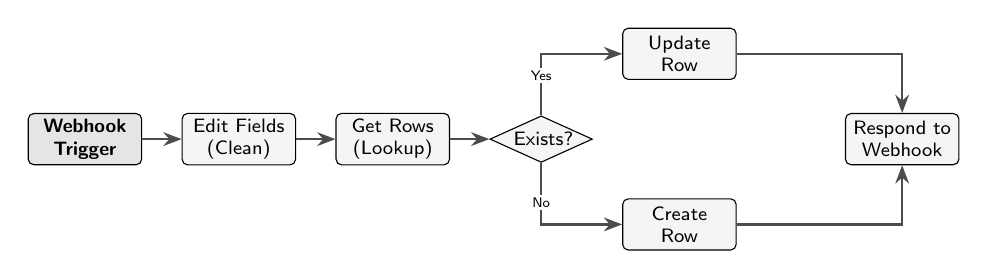
\begin{tikzpicture}[node distance=0.4cm and 0.5cm, align=center]
  \node (n1) [wf trigger] {Webhook\\Trigger};
  \node (n2) [wf node, right=of n1] {Edit Fields\\(Clean)};
  \node (n3) [wf node, right=of n2] {Get Rows\\(Lookup)};
  \node (n4) [wf decision, right=of n3] {Exists?};
  \node (n5a) [wf node, above right=0.6cm and 0.7cm of n4] {Update\\Row};
  \node (n5b) [wf node, below right=0.6cm and 0.7cm of n4] {Create\\Row};
  \node (n6) [wf node, right=3.2cm of n4] {Respond to\\Webhook};

  \draw [wf arrow] (n1) -- (n2);
  \draw [wf arrow] (n2) -- (n3);
  \draw [wf arrow] (n3) -- (n4);
  \draw [wf arrow] (n4) |- node[wf label, pos=0.25, above] {Yes} (n5a);
  \draw [wf arrow] (n4) |- node[wf label, pos=0.25, below] {No} (n5b);
  \draw [wf arrow] (n5a) -| (n6);
  \draw [wf arrow] (n5b) -| (n6);
\end{tikzpicture}%
}
\caption{WF-01: Data Ingestion Pipeline.}
\label{fig:wf01}
\end{figure}

\textbf{WF-02: Stockout Date Calculator} fetches all products, applies the stockout prediction formula from (\ref{eq:stockout_days}), and updates each product record with \texttt{days\_to\_stockout} and \texttt{estimated\_stockout\_date}.

\begin{figure}[H]
\centering
\resizebox{\columnwidth}{!}{%
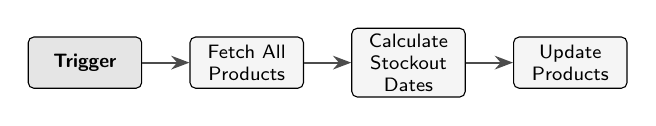
\begin{tikzpicture}[node distance=0.4cm and 0.6cm, align=center]
  \node (n1) [wf trigger] {Trigger};
  \node (n2) [wf node, right=of n1] {Fetch All\\Products};
  \node (n3) [wf node, right=of n2] {Calculate\\Stockout Dates};
  \node (n4) [wf node, right=of n3] {Update\\Products};

  \draw [wf arrow] (n1) -- (n2);
  \draw [wf arrow] (n2) -- (n3);
  \draw [wf arrow] (n3) -- (n4);
\end{tikzpicture}%
}
\caption{WF-02: Stockout Prediction Pipeline.}
\label{fig:wf02}
\end{figure}

\textbf{WF-03: Inventory Processing \& Stock Alerts} identifies products where \texttt{current\_stock} $\leq$ \texttt{reorder\_threshold}, clears existing alerts, and generates fresh Stock Alert records.

\begin{figure}[H]
\centering
\resizebox{\columnwidth}{!}{%
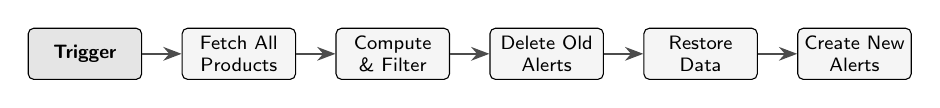
\begin{tikzpicture}[node distance=0.4cm and 0.5cm, align=center]
  \node (n1) [wf trigger] {Trigger};
  \node (n2) [wf node, right=of n1] {Fetch All\\Products};
  \node (n3) [wf node, right=of n2] {Compute\\\& Filter};
  \node (n4) [wf node, right=of n3] {Delete Old\\Alerts};
  \node (n5) [wf node, right=of n4] {Restore\\Data};
  \node (n6) [wf node, right=of n5] {Create New\\Alerts};

  \draw [wf arrow] (n1) -- (n2);
  \draw [wf arrow] (n2) -- (n3);
  \draw [wf arrow] (n3) -- (n4);
  \draw [wf arrow] (n4) -- (n5);
  \draw [wf arrow] (n5) -- (n6);
\end{tikzpicture}%
}
\caption{WF-03: Inventory Processing \& Alerts Pipeline.}
\label{fig:wf03}
\end{figure}

\textbf{WF-04: Stock Risk Classification} classifies all products into risk tiers using the formula in (\ref{eq:risk_classification}) based on \texttt{days\_to\_stockout} values from WF-02.

\begin{figure}[H]
\centering
\resizebox{\columnwidth}{!}{%
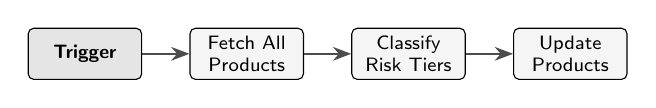
\begin{tikzpicture}[node distance=0.4cm and 0.6cm, align=center]
  \node (n1) [wf trigger] {Trigger};
  \node (n2) [wf node, right=of n1] {Fetch All\\Products};
  \node (n3) [wf node, right=of n2] {Classify\\Risk Tiers};
  \node (n4) [wf node, right=of n3] {Update\\Products};

  \draw [wf arrow] (n1) -- (n2);
  \draw [wf arrow] (n2) -- (n3);
  \draw [wf arrow] (n3) -- (n4);
\end{tikzpicture}%
}
\caption{WF-04: Risk Classification Pipeline.}
\label{fig:wf04}
\end{figure}

\textbf{WF-05: AI Reorder Intelligence} fetches at-risk products and all suppliers, then invokes Groq Llama 3.1 8B with a structured prompt to generate reorder recommendations. The LLM output is parsed and stored as Reorder Suggestions.

\begin{figure}[H]
\centering
\resizebox{\columnwidth}{!}{%
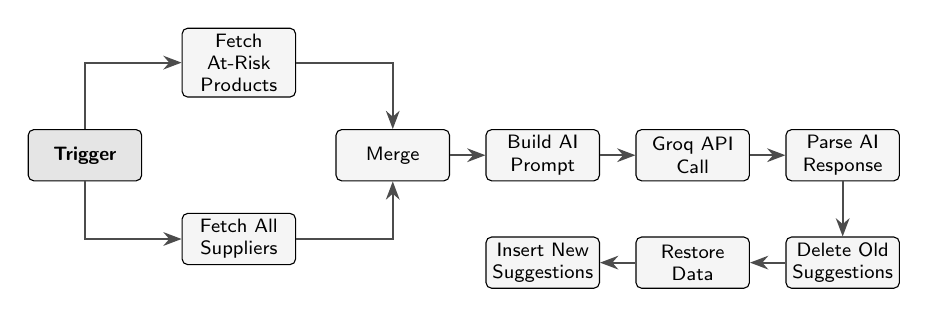
\begin{tikzpicture}[node distance=0.4cm and 0.45cm, align=center]
  % Row 1: Trigger -> parallel fetch -> merge -> prompt -> groq -> parse
  \node (n1) [wf trigger] {Trigger};
  \node (n2a) [wf node, above right=0.4cm and 0.5cm of n1] {Fetch At-Risk\\Products};
  \node (n2b) [wf node, below right=0.4cm and 0.5cm of n1] {Fetch All\\Suppliers};
  \node (n3) [wf node, below right=0.4cm and 0.5cm of n2a] {Merge};
  \node (n4) [wf node, right=of n3] {Build AI\\Prompt};
  \node (n5) [wf node, right=of n4] {Groq API\\Call};
  \node (n6) [wf node, right=of n5] {Parse AI\\Response};
  % Row 2: delete -> restore -> create
  \node (n7) [wf node, below=0.7cm of n6] {Delete Old\\Suggestions};
  \node (n8) [wf node, left=of n7] {Restore\\Data};
  \node (n9) [wf node, left=of n8] {Insert New\\Suggestions};

  \draw [wf arrow] (n1) |- (n2a);
  \draw [wf arrow] (n1) |- (n2b);
  \draw [wf arrow] (n2a) -| (n3);
  \draw [wf arrow] (n2b) -| (n3);
  \draw [wf arrow] (n3) -- (n4);
  \draw [wf arrow] (n4) -- (n5);
  \draw [wf arrow] (n5) -- (n6);
  \draw [wf arrow] (n6) -- (n7);
  \draw [wf arrow] (n7) -- (n8);
  \draw [wf arrow] (n8) -- (n9);
\end{tikzpicture}%
}
\caption{WF-05: AI Reorder Intelligence Pipeline.}
\label{fig:wf05}
\end{figure}

\textbf{WF-06: Supplier Scoring} evaluates all suppliers using the WSM formula from (\ref{eq:supplier_scoring}), computes composite scores, and assigns letter grades.

\begin{figure}[H]
\centering
\resizebox{\columnwidth}{!}{%
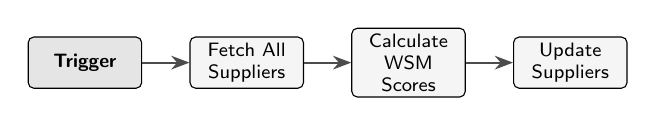
\begin{tikzpicture}[node distance=0.4cm and 0.6cm, align=center]
  \node (n1) [wf trigger] {Trigger};
  \node (n2) [wf node, right=of n1] {Fetch All\\Suppliers};
  \node (n3) [wf node, right=of n2] {Calculate\\WSM Scores};
  \node (n4) [wf node, right=of n3] {Update\\Suppliers};

  \draw [wf arrow] (n1) -- (n2);
  \draw [wf arrow] (n2) -- (n3);
  \draw [wf arrow] (n3) -- (n4);
\end{tikzpicture}%
}
\caption{WF-06: Supplier Scoring Pipeline.}
\label{fig:wf06}
\end{figure}

\textbf{WF-07: WhatsApp Alert Sender} queries active stock alerts, filters by 24-hour anti-spam cooldown, builds a formatted message, and delivers it via Twilio WhatsApp API.

\begin{figure}[H]
\centering
\resizebox{\columnwidth}{!}{%
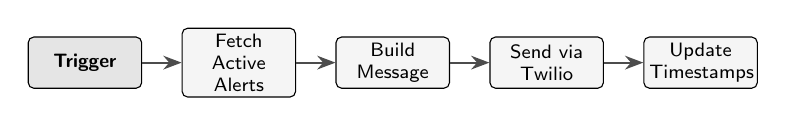
\begin{tikzpicture}[node distance=0.4cm and 0.5cm, align=center]
  \node (n1) [wf trigger] {Trigger};
  \node (n2) [wf node, right=of n1] {Fetch Active\\Alerts};
  \node (n3) [wf node, right=of n2] {Build\\Message};
  \node (n4) [wf node, right=of n3] {Send via\\Twilio};
  \node (n5) [wf node, right=of n4] {Update\\Timestamps};

  \draw [wf arrow] (n1) -- (n2);
  \draw [wf arrow] (n2) -- (n3);
  \draw [wf arrow] (n3) -- (n4);
  \draw [wf arrow] (n4) -- (n5);
\end{tikzpicture}%
}
\caption{WF-07: WhatsApp Alert Pipeline.}
\label{fig:wf07}
\end{figure}

\textbf{WF-08: Daily Orchestrator} is the master workflow executing at 8:00 AM IST. It simulates daily stock depletion, sequentially executes WF-02 through WF-07 as sub-workflows, computes and saves the daily health snapshot, and logs execution to System Logs.

\begin{figure}[H]
\centering
\resizebox{\columnwidth}{!}{%
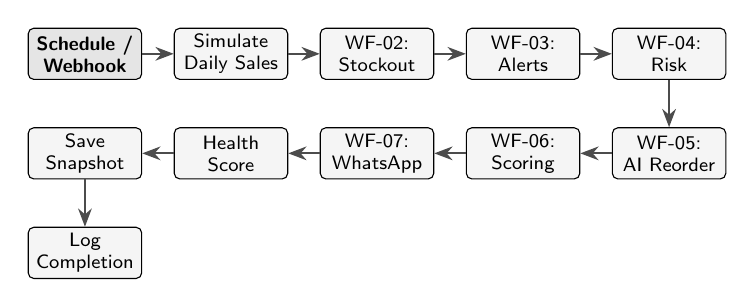
\begin{tikzpicture}[node distance=0.35cm and 0.4cm, align=center]
  % Row 1: Triggers -> Simulate -> WF-02 -> WF-03 -> WF-04
  \node (trig) [wf trigger] {Schedule /\\Webhook};
  \node (sim) [wf node, right=of trig] {Simulate\\Daily Sales};
  \node (w2) [wf node, right=of sim] {WF-02:\\Stockout};
  \node (w3) [wf node, right=of w2] {WF-03:\\Alerts};
  \node (w4) [wf node, right=of w3] {WF-04:\\Risk};
  % Row 2: WF-05 -> WF-06 -> WF-07 -> Snapshot -> Log
  \node (w5) [wf node, below=0.6cm of w4] {WF-05:\\AI Reorder};
  \node (w6) [wf node, left=of w5] {WF-06:\\Scoring};
  \node (w7) [wf node, left=of w6] {WF-07:\\WhatsApp};
  \node (score) [wf node, left=of w7] {Health\\Score};
  \node (snap) [wf node, left=of score] {Save\\Snapshot};
  % Row 3
  \node (log) [wf node, below=0.6cm of snap] {Log\\Completion};

  \draw [wf arrow] (trig) -- (sim);
  \draw [wf arrow] (sim) -- (w2);
  \draw [wf arrow] (w2) -- (w3);
  \draw [wf arrow] (w3) -- (w4);
  \draw [wf arrow] (w4) -- (w5);
  \draw [wf arrow] (w5) -- (w6);
  \draw [wf arrow] (w6) -- (w7);
  \draw [wf arrow] (w7) -- (score);
  \draw [wf arrow] (score) -- (snap);
  \draw [wf arrow] (snap) -- (log);
\end{tikzpicture}%
}
\caption{WF-08: Master Daily Orchestrator Pipeline.}
\label{fig:wf08}
\end{figure}

\textbf{WF-09: AI Vision Onboarding} exposes a webhook for the Smart Scan feature. It accepts base64-encoded image data from the frontend, prompts Google Gemini 2.5 Flash to extract product details (name, category), generates a collision-free sequential ID using existing database records, and returns structured JSON to auto-fill the product form.

\begin{figure}[H]
\centering
\resizebox{\columnwidth}{!}{%
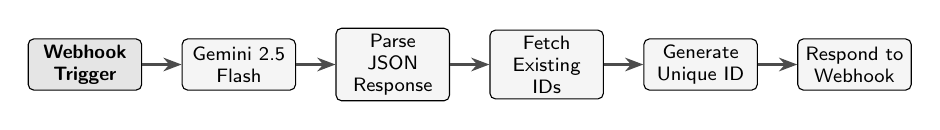
\begin{tikzpicture}[node distance=0.4cm and 0.5cm, align=center]
  \node (n1) [wf trigger] {Webhook\\Trigger};
  \node (n2) [wf node, right=of n1] {Gemini 2.5\\Flash};
  \node (n3) [wf node, right=of n2] {Parse JSON\\Response};
  \node (n4) [wf node, right=of n3] {Fetch Existing\\IDs};
  \node (n5) [wf node, right=of n4] {Generate\\Unique ID};
  \node (n6) [wf node, right=of n5] {Respond to\\Webhook};

  \draw [wf arrow] (n1) -- (n2);
  \draw [wf arrow] (n2) -- (n3);
  \draw [wf arrow] (n3) -- (n4);
  \draw [wf arrow] (n4) -- (n5);
  \draw [wf arrow] (n5) -- (n6);
\end{tikzpicture}%
}
\caption{WF-09: AI Vision Onboarding Pipeline.}
\label{fig:wf09}
\end{figure}

\textbf{WF-10: Smart Scan for Supplier Invoices} processes photos of physical delivery bills to automate inventory intake. It uses Gemini 2.5 Flash to extract product names and quantities, then performs fuzzy matching against the existing inventory database to compute and update the new stock levels.

\begin{figure}[H]
\centering
\resizebox{\columnwidth}{!}{%
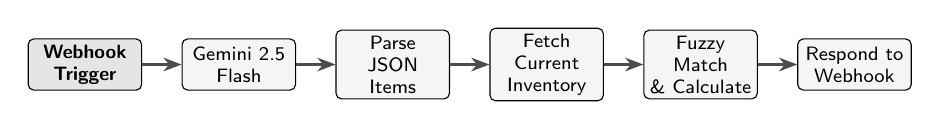
\begin{tikzpicture}[node distance=0.4cm and 0.5cm, align=center]
  \node (n1) [wf trigger] {Webhook\\Trigger};
  \node (n2) [wf node, right=of n1] {Gemini 2.5\\Flash};
  \node (n3) [wf node, right=of n2] {Parse JSON\\Items};
  \node (n4) [wf node, right=of n3] {Fetch Current\\Inventory};
  \node (n5) [wf node, right=of n4] {Fuzzy Match\\\& Calculate};
  \node (n6) [wf node, right=of n5] {Respond to\\Webhook};

  \draw [wf arrow] (n1) -- (n2);
  \draw [wf arrow] (n2) -- (n3);
  \draw [wf arrow] (n3) -- (n4);
  \draw [wf arrow] (n4) -- (n5);
  \draw [wf arrow] (n5) -- (n6);
\end{tikzpicture}%
}
\caption{WF-10: Smart Scan Invoice Pipeline.}
\label{fig:wf10}
\end{figure}

\subsection{LLM Prompt Engineering}

WF-05 constructs a structured prompt submitted to the 
Groq Llama~3.1~8B inference endpoint. The prompt 
follows a zero-shot instruction format comprising three 
components: (1)~a role definition establishing the 
model as an inventory manager for an Indian kirana store; 
(2)~structured context blocks listing at-risk products 
with fields \texttt{product\_id}, \texttt{category}, 
\texttt{current\_stock}, \texttt{avg\_daily\_sales}, 
\texttt{days\_to\_stockout}, and \texttt{risk\_level}; 
and (3)~available supplier profiles with 
\texttt{supplier\_id}, \texttt{supplier\_grade}, 
\texttt{delivery\_time\_days}, and 
\texttt{supplies\_categories}.

The model is instructed to output a JSON array 
with no markdown fencing or natural language preamble. 
Each element contains product id, 
supplier id, suggested qty
(calculated as $30 \times v$ where $v$ is average daily 
sales), and a reason field providing a 
single sentence justification for the suggestion it generated.

For WF-09, a separate prompt instructs Google Gemini 2.5 Flash to analyze a base64-encoded image of a product and extract its \texttt{product\_name} and \texttt{category}. A recursive parser handles the multimodal response to correctly extract the structured JSON payload, enabling automated data entry.

For WF-10, the prompt directs the LLM to identify all line items on a supplier invoice, specifically extracting product names and total delivered quantities. The resulting JSON is then passed to a code-based fuzzy matching algorithm that maps these items to the store's specific \texttt{product\_id} schema by calculating string similarity scores against the active inventory table.

\subsection{Frontend Application}

The React 19 frontend provides the main application pages described in Table~\ref{tab:routes}.

\begin{table}[htbp]
\centering
\caption{Frontend Pages and Functions}
\label{tab:routes}
\begin{tabular}{p{2.2cm}p{5.5cm}}
\toprule
\textbf{Page} & \textbf{Function} \\
\midrule
/ & Landing page \\
/login, /signup & Supabase Auth entry points \\
/reset-password & Password reset flow \\
/onboarding & 3-step store setup wizard \\
/dashboard & Health score, KPIs, critical products, trend chart \\
/products & Product CRUD, CSV bulk import, and AI Smart Scan \\
/quick-update & Batch stock adjustments \\
/alerts & Stock alert feed with dismiss \\
/reorder & AI reorder suggestions with approve/dismiss \\
/suppliers & Supplier table with grade badges \\
/logs & System log viewer \\
/settings & Store profile and workflow triggers \\
\bottomrule
\end{tabular}
\end{table}

Once the run pipeline button is triggered the user can see a animated overlay of pipeline processing that is taking place in the backend. If the pipeline completes the processing successfully then the user can see a green success message and automatically updated dashboard whereas if the pipeline fails then the user can see a failure message in red.

\section{Results and Performance}


The implemented system was tested using a sample data consisting of 10 different products mapped against 4 different suppliers. The key performance metrics are summarized in the Table~\ref{tab:perf}.

\begin{table}[htbp]
\centering
\caption{System Performance Metrics}
\label{tab:perf}
\begin{tabular}{lc}
\toprule
\textbf{Metric} & \textbf{Value} \\
\midrule
Number of Workflows & 10 \\
Number of Database Tables & 8 \\
Number of Main Frontend Pages & 12 \\
Pipeline Execution Time & $\sim$13 seconds \\
WhatsApp Message Delivery & $<$5 seconds \\
Infrastructure Cost & Rs.\ 0 (prototype); $<$Rs.\ 500/mo (production) \\
\bottomrule
\end{tabular}
\end{table}

Table IV presents a comparative analysis of StockSense AI 
against existing inventory management solutions available 
to small Indian retailers. The comparison shows the unique features 
of StockSense AI compared to other existing products in the market.

\begin{table}[htbp]
\centering
\caption{Comparison with Existing Inventory Solutions}
\label{tab:comparison}
\renewcommand{\arraystretch}{1.4}
\begin{tabularx}{\columnwidth}{lXXXX}
\toprule
\textbf{Feature} & \textbf{StockSense AI} & \textbf{Vyapar} & \textbf{Zoho Inventory} & \textbf{Khatabook} \\
\midrule
AI Reorder Suggestions & Yes & No & Limited & No \\
Stockout Prediction & Automated & Manual & Basic & No \\
Supplier Scoring & WSM-based & No & Basic & No \\
WhatsApp Alerts & Automated & No & No & No \\
Monthly Cost & Rs. 0--500 & Rs. 0--599 & Rs. 4,000+ & Rs. 0 \\
Setup Complexity & Low & Medium & High & Low \\
Prediction Method & Rule-based & No & Basic & No \\
Real-time Dashboard & Yes & Limited & Yes & No \\
\bottomrule
\end{tabularx}
\end{table}

\subsection*{Health Score Validation}
In order to validate the health score formula defined in (5), 
the system was evaluated across four different inventory states 
that represents some of the typical real time scenarios
in the kriana stores. 
The table V contains the computed scores for each of the scenarios.

\begin{table}[htbp]
\centering
\caption{Health Score Across Inventory States}
\label{tab:healthscores}
\renewcommand{\arraystretch}{1.4}
\begin{tabular}{lcccccc}
\toprule
\textbf{Scenario} & $n_L$ & $n_M$ & $n_H$ & $n_O$ & $N$ & $H$ \\
\midrule
All well-stocked   & 10 & 0 & 0 & 0 & 10 & 100 \\
Demo state         & 3  & 1 & 6 & 0 & 10 & 55  \\
Severe stockout    & 0  & 2 & 0 & 8 & 10 & 18  \\
Complete stockout  & 0  & 0 & 0 & 10 & 10 & 5   \\
\bottomrule
\end{tabular}
\end{table}

Some of the key findings from the table which validates
real world scenarios are: the fully stocked store scenario
has a perfect score of 100 whereas the store with 3 oos 
products has a score of 18 that shows the need of 
critical intervention.

The prototype operates on free tier and sandboxed services like: Supabase , Groq, and N8N. The twilio WhatsApp is validated in sandbox environment mode during the development phase. For production deployment, n8n requires cloud hosting (approximately Rs.300 to 500/month on platforms such as Railway or Render), and the Twilio WhatsApp Business API incurs nominal charges/message. Even with these costs, the total monthly expenditure for a single store remains under Rs.500 which is practically affordable and useful for a small scale shop owner.

The automated daily pipeline successfully orchestrates all sub workflows in sequence, processing all products and generating alerts without manual intervention. If the workflow engine is actively hosted in a cloud platform the shop owners can get the daily intelligence report at a specific time as per their 
choice based on the individual specific needs using the N8N's built in cron trigger option that fires the pipeline automatically at a particular time.

The WhatsApp alert feature helps the shop owners in receiving stock alerts once the pipeline is triggered and it acts a simple yet effective source of information as most of the kirana shop owners in India will be using WhatsApp on a daily basis and it will be more convenient compared to SMS or mail notifications. The 24 hours anti spam cooldown feature ensure that the critical alerts are delivered promptly and service stays active.

The health score on the main dashboard shows a score between 0 to 100 that shows the current state of the inventory and weighted formula correctly penalises the oos and high risk products whereas rewarding the well stocked products.

The AI based reorder suggestion using the Groq Llama 3.1 8B provides really useful and simple recommendations in natural language that considers the product details, supplier capabilities, and current stock levels. It also helps the store owners in understanding the reason behind a particular suggestion generated.

\section{Conclusion}

Hence, we discussed the detailed architecture and usage of the project StockSense AI in this paper. It clearly shows that this simple system helps small scale shop owners to track and manage their inventory in an efficient way with the help of advanced features that are available at a minimal cost compares to costly exisitng ERP solutions in the market.

The system successfully integrates 5 key technical parts like automated stockout prediction using daily sales velocity, AI-driven reorder recommendations via Groq Llama 3.1 8B, multi criteria supplier scoring using the Weighted Sum Model, real time WhatsApp alerts via Twilio, and fully orchestrated workflows in N8N. All of this operates at under Rs.500/month which is really cheaper and affordable for small scale shop owners compared to exising costly softwares.

From the implementation perspective the usage of low code automation framework N8N was really useful as it helped in developing the complete backend as well as the business logics in a simple way compared to traditional coding method. This also shows that latest technologies like N8N is really helput in business automation's where time to market and cost efficiency plays a critical role in the operations.

However current design and the overall system consists of several limitations that need to be disccused. First, the stock out prediction depends on historical daily sales velocity and assuems that the demand pattern remains relatively stable, it won't capture sudden seasonal spikes or situations like festivals etc. unless an extra context is provided. Second, the weigthed sum model which is used for supplier scoring is deterministic and it doesn't learn from historical performance feedbacks. Third, the current implementation is for a single store setup, inorder to facilitate multi stores capability we have enable row level security for the database tables and redesign the overall database schema.

Hence the project shows that with the help of latest technologies it is practically possible to develop simple but effective solutions to various business problems in much more cheaper way compared to traditional software development. StockSense AI is a practical and effective tool for kirana shop owners helping them in solving some of their biggest headaches related to inventory management

\section{Future Scope}

\label{sec:future}

The present system is a working prototype or proof of concept. Some of the future improvements in consideration are:

\textbf{Mobile App:} Since most of the small scale shope owners uses mobile as part of their daily life, hence it will be ideal to develop the mobile app version of this project.

\textbf{Regional languages support:} Since India is a vast country with lot's of languages it will be ideal to cover as much regional languages possible inorder to cater to a large number of users.

\textbf{Two-way WhatsApp:} This feature would let the shop owners reply to the alerts that they revieve in WhatsApp and proceed to next stage without the need of logging into the app. 

The schema has fields for seasonal tracking. During festivals, a seasonal multiplier could adjust demand estimates for accuracy around Diwali, Holi, and harvest season.

\textbf{Multi-store support:} This can be facilitated with advanced database modelling and schema design.

\textbf{Purchase order generation:} This will process the reorder suggestions that are approved to the next stage of actual purchase which involves contacting suppliers and facilitation UPI payments automatically.

\begin{thebibliography}{10}

\bibitem{inventory2024}
J. Wang, P. Li, L. Luo and H . Sun, ``Design and Development of Intelligent Inventory System for Small and Micro Enterprise Warehousing,'' \emph{IEEE Conf. on Computer, Big Data and AI}, 2024. [Online]. Available: \url{https://ieeexplore.ieee.org/document/10550978/}

\bibitem{forecasting2023}
N. Kheawpeam and S. Sinthupinyo, ``Demand Forecasting Using Machine Learning to Manage Product Inventory for Multi-channel Retailing Store,'' \emph{IEEE Int. Conf. on Omni-layer Intelligent Systems}, 2023. [Online]. Available: \url{https://ieeexplore.ieee.org/document/10189241/}

\bibitem{retail2024}
Jaymin V. Soni and Chetansinh Vaghela, ``Retail Demand Forecasting in Inventory with External Influences: A Comparative Study of Machine Learning Models,'' \emph{IEEE Trans. on Retail Tech.}, 2024. [Online]. Available: \url{https://ieeexplore.ieee.org/document/11232957/}

\bibitem{llm2024}
Mohammad Al Khaldy and Youcef Gheraibia, ``Evaluation and Mitigation of the Limitations of Large Language Models in Business Decision-Making,'' \emph{IEEE Access}, 2024. [Online]. Available: \url{https://ieeexplore.ieee.org/document/11013278/}

\bibitem{cognitive2025}
Natalie Friedman, Marcus Krug. and S. Joy Mountford, ``Mediating Cognitive Biases in Business Decisions Using LLMs,'' \emph{IEEE Trans. on AI}, 2025. [Online]. Available: \url{https://ieeexplore.ieee.org/document/11050471/}

\bibitem{workflow2025}
Ahmed Raza Amir and Syed Muhammad Atif, ``Evaluating Workflow Automation Efficiency Using n8n: A Small-Scale Business Case Study,'' \emph{arXiv preprint arXiv:2602.01311}, Feb. 2025. [Online]. Available: \url{https://arxiv.org/abs/2602.01311}

\bibitem{msme2019}
Dinesh Shenoy and Hoshiar Mal, ``A Multi-item Inventory Model for Small Business---A Perspective from India,'' \emph{Int. J. of Inventory Research}, vol.~5, no.~3, pp.~188--209, 2019. [Online]. Available: \url{https://www.inderscienceonline.com/doi/abs/10.1504/IJIR.2019.098856}

\bibitem{iot2024}
Geetha Manoharan, Vipin Kumar, A Karthik, V Asha, Chinnem Rama Mohan, and Ginni Nijhawan, ``IoT-Based Smart Inventory Management System Using Machine Learning Techniques,'' \emph{IEEE Internet of Things Journal}, 2024. [Online]. Available: \url{https://ieeexplore.ieee.org/document/10601903/}

\bibitem{smartretail2024}
K. Poongothai, Devika. G, Sweety Brisila. D, and Yogesh. S, ``Smart Retail Using Machine Learning for Demand Forecasting and Inventory Optimization,'' \emph{IEEE Trans. on Smart Business}, 2024. [Online]. Available: \url{https://ieeexplore.ieee.org/document/10910874/}

\bibitem{n8n2025}
Padmanabhan Venkiteela, ``n8n: An Open-Source Workflow Automation Platform for Enterprise Integration and AI-Driven Orchestration,'' \emph{Int. J. of Computer Applications}, vol.~187, no.~63, Dec.~2025. [Online]. Available: \url{https://www.ijcaonline.org/archives/volume187/number63/}

\end{thebibliography}

\end{document}
